\documentclass[11pt,a4paper]{article}
\usepackage{iftex}
\ifPDFTeX
  \usepackage[T1]{fontenc}
  \usepackage[utf8]{inputenc}
\else
  \usepackage{fontspec}
\fi
\usepackage[spanish,es-noshorthands]{babel}
\usepackage{amsmath,amssymb}
\usepackage{booktabs}
\usepackage{graphicx}
\usepackage{geometry}
\usepackage{caption}
\usepackage{float}
\usepackage{hyperref}
\geometry{margin=2.35cm}
\graphicspath{{../results/comparacion/graficas/}}
\emergencystretch=2em
\hypersetup{colorlinks=true,linkcolor=black,urlcolor=blue}
\captionsetup{font=small,skip=6pt,labelfont=bf}
\renewcommand{\topfraction}{0.92}
\renewcommand{\bottomfraction}{0.85}
\renewcommand{\textfraction}{0.07}
\renewcommand{\floatpagefraction}{0.8}
\setcounter{topnumber}{2}
\setcounter{totalnumber}{3}
\title{Comparación de Tersoff y LCBOPII\\[0.35em]
\large Mismo Monte Carlo, dos potenciales}
\author{Emanuel Orozco Gallego}
\date{18 de noviembre de 2026}
\begin{document}
\maketitle

\begin{abstract}
Los dos informes anteriores corren el mismo Monte Carlo del paper de Fasolino, Los y Katsnelson (2007).
Cambia el potencial.
Tersoff tiene las cinco cajas hasta $N=8640$.
LCBOPII tiene cuatro, hasta $N=4860$, porque $N=8640$ se detuvo.
El error se calcula en las cuatro cajas comunes.
En el enlace, LCBOPII queda a $0.4\%$ de $1.42\,\text{\AA}$ y Tersoff entre $1.1\%$ y $1.8\%$.
En $G(q)$, entre $q=0.20$ y $0.40\,\text{\AA}^{-1}$, LCBOPII está a un $9\%$ de $G_0$ y Tersoff un $43\%$ por debajo.
Hacia $q\sim 1\,\text{\AA}^{-1}$ la relación se invierte: Tersoff queda más cerca de la recta del paper.
Para seguir el artículo conviene LCBOPII.
Tersoff sigue siendo el control rápido de la receta.
\end{abstract}

\tableofcontents

\section{Qué comparten y qué no}

Las dos campañas empiezan en la hoja plana, a $300\,\mathrm{K}$, con el movimiento de Metrópolis.
Un paso son $N$ intentos y cada cinco pasos hay un cambio de área.
El equilibrado dura $4\times 10^5$ pasos y la producción $5\times 10^5$.
Las cajas salen de la misma fórmula, $L_x=p|a_1|$ y $L_y=q\cdot 3a$, con $a=1.42\,\text{\AA}$.
$G(q)$, $g(r)$ y $h_{\mathrm{rms}}$ se definen igual.
$G_0$ usa $\kappa=1.1\,\mathrm{eV}$.

Tersoff es el de Lindsay y Broido.
Mira vecinos hasta $2.10\,\text{\AA}$ y no tiene canal de conjugación.
LCBOPII es el potencial del paper.
Mira hasta $6\,\text{\AA}$ e incluye conjugación, torsión y alcance medio.
Su hoja plana da $-7.350\,\mathrm{eV}$ por átomo.
La de Tersoff da $-7.966\,\mathrm{eV}$ por átomo.
Esas dos energías no se restan entre sí: cada potencial tiene su cero.

La comparación cuantitativa usa $N=240$, $960$, $2160$ y $4860$.
El $N=8640$ de Tersoff no tiene par en LCBOPII.

\section{Cómo se mide el error}

Hay dos errores distintos.

Contra el paper se usa un número que el artículo fija.
El enlace conjugado es $1.42\,\text{\AA}$, así que el error del pico de $g(r)$ es $(\text{pico}-1.42)/1.42$.
La recta armónica es $G_0$, así que el error de un tramo de $G(q)$ es la mediana de $G/G_0$ menos uno.
Un valor negativo queda por debajo de la recta.

Entre los dos métodos, el error relativo de una magnitud $x$ es $(x_{\mathrm{L}}-x_{\mathrm{T}})/x_{\mathrm{T}}$.
La energía total no entra en esa cuenta, porque los ceros son distintos.
Sí entra el exceso sobre el cristal de cada potencial: la hoja tibia menos la hoja plana.

\section{Error entre los dos métodos}

\begin{table}[ht]
\centering
\small
\caption{Altura y enlace en las cuatro cajas comunes.
$h$ está en \AA.
El error de $h$ es $(h_{\mathrm{L}}-h_{\mathrm{T}})/h_{\mathrm{T}}$.
El error del pico es contra $1.42\,\text{\AA}$.}
\begin{tabular}{rrrrrr}
\toprule
$N$ & $h$ Tersoff & $h$ LCBOPII & error de $h$ & pico T & pico L \\
\midrule
240  & $0.180\pm 0.007$ & $0.245\pm 0.009$ & $+37\%$ & 1.435 & 1.425 \\
960  & $0.318\pm 0.021$ & $0.385\pm 0.028$ & $+21\%$ & 1.435 & 1.425 \\
2160 & $0.385\pm 0.016$ & $0.500\pm 0.045$ & $+30\%$ & 1.435 & 1.425 \\
4860 & $0.473\pm 0.025$ & $0.501\pm 0.028$ & $+6\%$  & 1.445 & 1.425 \\
\bottomrule
\end{tabular}
\end{table}

LCBOPII ondula más en las cajas chicas.
En $N=4860$ las dos alturas ya se tocan dentro de la dispersión de las réplicas: $0.47$ y $0.50\,\text{\AA}$.
Las dos se frenan al crecer la caja. LCBOPII se frena antes.

\begin{figure}[H]
\centering
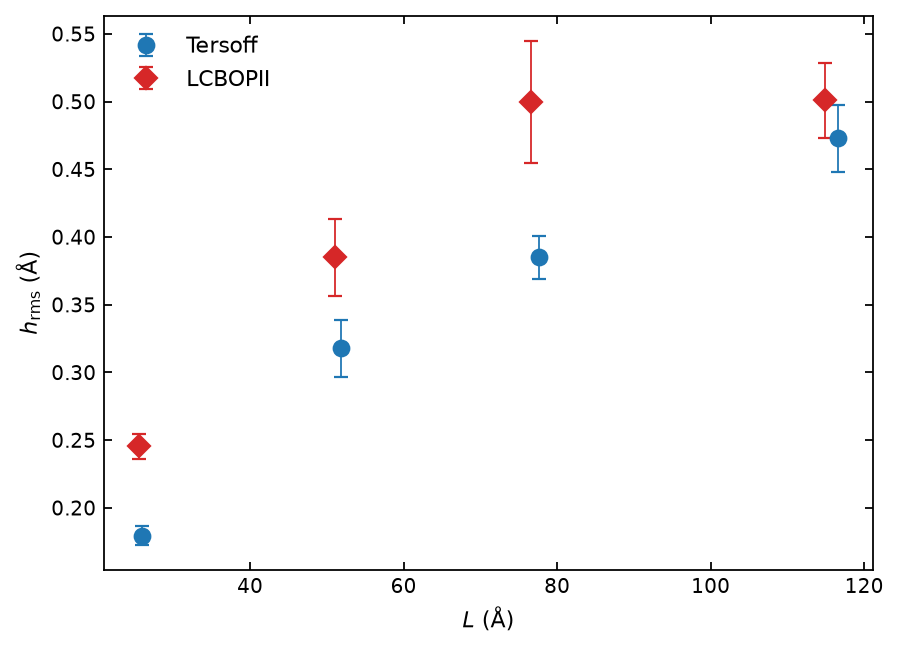
\includegraphics[width=0.70\textwidth]{hrms_comparacion.png}
\caption{Altura de las cuatro cajas comunes.
Los círculos son Tersoff y los rombos son LCBOPII.
La barra es la dispersión entre réplicas.}
\end{figure}

El pico de Tersoff está $0.015\,\text{\AA}$ por encima de $1.42\,\text{\AA}$ en las tres cajas chicas, un $1.1\%$, y $0.025\,\text{\AA}$ en $N=4860$, un $1.8\%$.
El de LCBOPII está $0.005\,\text{\AA}$ por encima en las cuatro, un $0.4\%$.
Ninguno abre hombros en $1.31$ ni en $1.54\,\text{\AA}$.
Esos hombros, en el paper, aparecen a $3500\,\mathrm{K}$.

\begin{figure}[H]
\centering
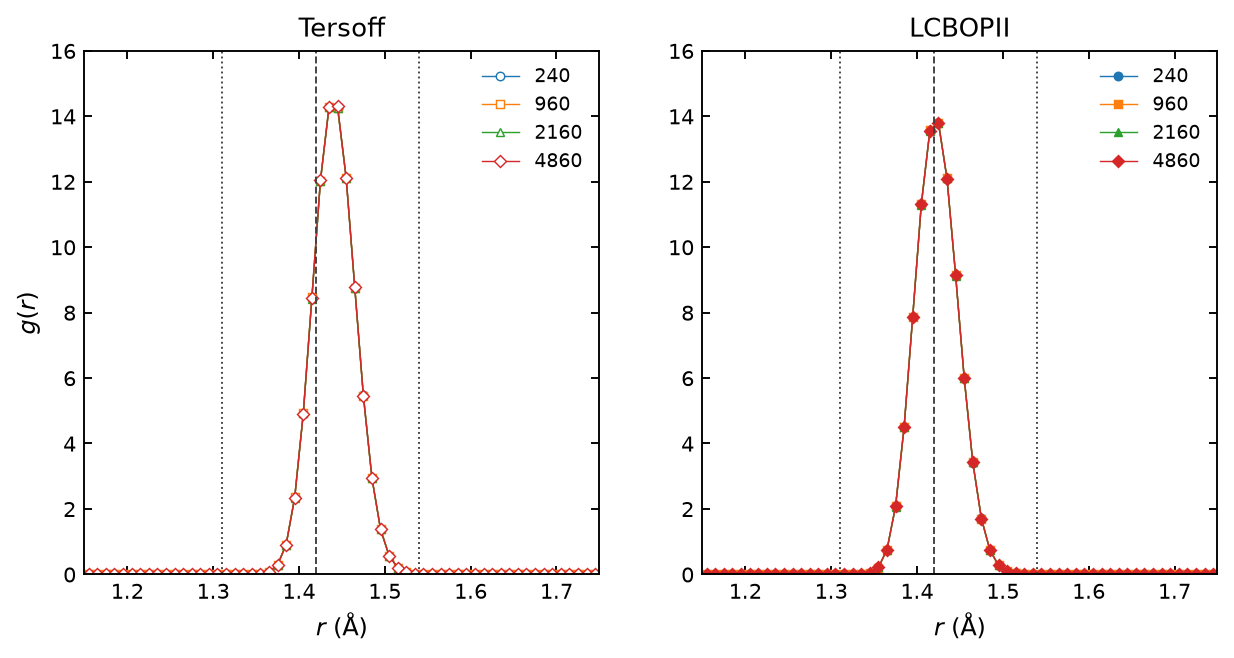
\includegraphics[width=\textwidth]{rdf_comparacion.png}
\caption{Primer pico de $g(r)$.
Las marcas son $1.31$, $1.42$ y $1.54\,\text{\AA}$.
Tersoff cae a la derecha de $1.42\,\text{\AA}$.
LCBOPII cae sobre esa marca.
Los cuatro tamaños de cada potencial coinciden.}
\end{figure}

\begin{table}[ht]
\centering
\small
\caption{Error de $G/G_0$ contra la recta del paper.
La ventana está en $\text{\AA}^{-1}$.
El error es la mediana de $G/G_0$ menos uno.}
\begin{tabular}{lrrrr}
\toprule
ventana & Tersoff & error T & LCBOPII & error L \\
\midrule
$0.20$--$0.40$ & 0.57 & $-43\%$ & 1.09 & $+9\%$ \\
$0.40$--$1.20$ & 0.74 & $-26\%$ & 1.71 & $+71\%$ \\
\bottomrule
\end{tabular}
\end{table}

Los cuatro tamaños dan casi el mismo cociente dentro de cada método, así que la tabla usa la media de las cuatro cajas.
El error de un método respecto del otro, $(G_{\mathrm{L}}-G_{\mathrm{T}})/G_{\mathrm{T}}$, es de cerca del $+91\%$ en la ventana $0.20$--$0.40$ y de cerca del $+131\%$ en $0.40$--$1.20$.

En las ondulaciones de unas decenas de ångströms, LCBOPII acompaña a $G_0$ y Tersoff se queda bajo.
Hacia $q\sim 1\,\text{\AA}^{-1}$ LCBOPII deja de caer como $1/q^2$ y Tersoff sigue más cerca de la recta, todavía por debajo, que es el lado en el que el paper dibuja sus curvas.
En la Fig.~3 del paper el fondo, justo antes del Bragg, baja hasta cerca de $2\times 10^{-3}$ y se apoya en $G_0$.
En $N=4860$, entre $q=1.2$ y $2.3\,\text{\AA}^{-1}$, la mediana es $5.7\times 10^{-3}$ con Tersoff y $1.3\times 10^{-2}$ con LCBOPII.
En $q=2\,\text{\AA}^{-1}$, $G_0$ vale $2.3\times 10^{-3}$.
Tersoff queda unas dos veces y media por encima de esa recta, y LCBOPII unas seis.
Ninguna de las dos llega al suelo de la figura del paper.
Ninguno de los dos muestra, con estas réplicas, el pico agudo de $70\,\text{\AA}$.
Los dos bajan $G/G_0$ en el modo más largo de $N=4860$: Tersoff a $0.10$ y LCBOPII también a $0.10$ en $q=0.056\,\text{\AA}^{-1}$.

\begin{figure}[H]
\centering
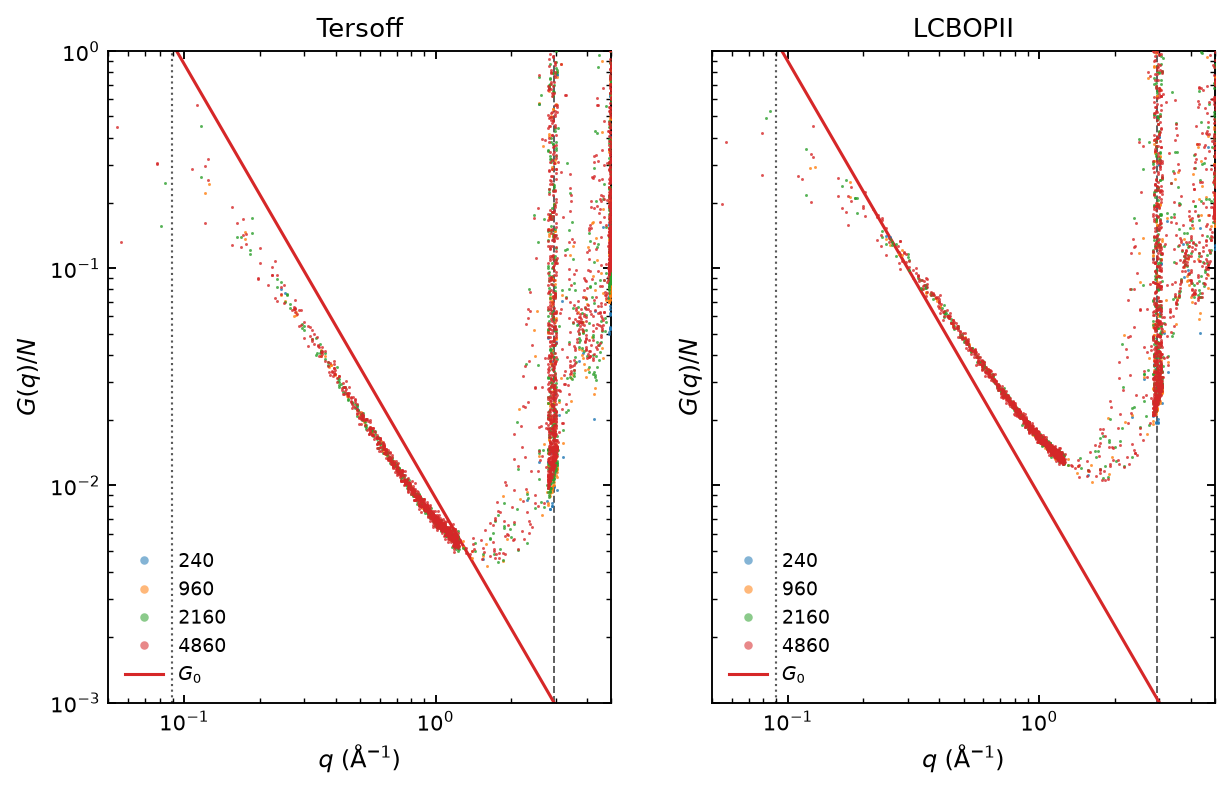
\includegraphics[width=\textwidth]{Gq_comparacion.png}
\caption{$G(q)/N$ en los ejes de la Fig.~3 del paper:
$q$ de $0.05$ a $5\,\text{\AA}^{-1}$ y $G/N$ de $10^{-3}$ a $1$.
Cada punto es un modo; no hay línea ni espaciado.
La recta roja es $G_0$.
La punteada marca los $70\,\text{\AA}$ y la discontinua el primer Bragg.}
\end{figure}

La aceptación fue del $39.2\%$ con Tersoff y del $43.0\%$ con LCBOPII.
El exceso de energía sobre el cristal propio es $27\,\mathrm{meV}$ por átomo con Tersoff y $37\,\mathrm{meV}$ por átomo con LCBOPII.
Los dos quedan por encima de su cristal, como corresponde a una hoja a $300\,\mathrm{K}$.

\section{Costo}

En Tersoff, la caja de $8640$ átomos daba un paso en $13\,\mathrm{ms}$ y esa lámina tardaba unas $3.3$ horas, con $32$ hilos.
LCBOPII, en $N=4860$ y con $16$ hilos por réplica, tardó unas $44$ horas de pared.
El corte de $6\,\text{\AA}$, la conjugación y la torsión hacen cada intento varias veces más caro, y dos átomos del mismo paso tienen que estar a más de $13\,\text{\AA}$ para evaluarse a la vez.
Ese costo es la razón de haber cerrado el estudio sin $N=8640$.

\section{Ventajas y límites}

Tersoff corre en horas, ya tiene la caja de $8640$ átomos y en la ventana ancha de la Fig.~3 se queda un poco por debajo de $G_0$, del lado del dibujo del paper.
Su límite es de fondo: sin el canal de conjugación no puede producir el máximo de $70\,\text{\AA}$ ni los hombros de $g(r)$, aunque se alargue la corrida.
El enlace queda en $1.44\,\text{\AA}$ y la energía no es la de la Tabla~II.

LCBOPII es el potencial con el que el paper hace la afirmación.
El enlace queda a $0.005\,\text{\AA}$ de $1.42\,\text{\AA}$, la hoja plana da la energía de la monocapa y, entre $0.20$ y $0.40\,\text{\AA}^{-1}$, $G(q)$ es el que más se acerca a $G_0$.
Su límite, en esta corrida, también es concreto.
Hacia $q\sim 1\,\text{\AA}^{-1}$ se va un $71\%$ por encima de la recta.
El pico de $70\,\text{\AA}$ no queda resuelto.
Faltan $N=8640$ y los $3500\,\mathrm{K}$ de las Figs.~4 y~5.
El tramo angular medio no es el polinomio publicado, que es discontinuo: es el empalme cúbico que deja el grafito plano como mínimo.

\section{Cuál implementar}

Para la pregunta del paper, el método es LCBOPII.
Tersoff no puede añadir el canal que el artículo usa para fijar los $70\,\text{\AA}$.
Para comprobar la receta, las cajas y la parte elástica en poco tiempo, el método es Tersoff, y ese control ya está hecho.

Si hay que seguir con uno solo, se sigue con LCBOPII: es el que puede acercarse a la Fig.~3 completa y, más adelante, a las Figs.~4 y~5.
Conviene terminarlo en $N=8640$ y mirar por qué, pasado $q\sim 0.4\,\text{\AA}^{-1}$, la curva se separa de $G_0$.
No conviene borrar Tersoff. Sirve de control, y en la ventana ancha de $G(q)$ hoy está más cerca del dibujo del paper que esta corrida de LCBOPII.

\end{document}
